\documentclass[14pt]{extbook}
\usepackage{multicol, enumerate, enumitem, hyperref, color, soul, setspace, parskip, fancyhdr} %General Packages
\usepackage{amssymb, amsthm, amsmath, bbm, latexsym, units, mathtools} %Math Packages
\everymath{\displaystyle} %All math in Display Style
% Packages with additional options
\usepackage[headsep=0.5cm,headheight=12pt, left=1 in,right= 1 in,top= 1 in,bottom= 1 in]{geometry}
\usepackage[usenames,dvipsnames]{xcolor}
\usepackage{dashrule}  % Package to use the command below to create lines between items
\newcommand{\litem}[1]{\item#1\hspace*{-1cm}\rule{\textwidth}{0.4pt}}
\pagestyle{fancy}
\lhead{Progress Quiz 9}
\chead{}
\rhead{Version B}
\lfoot{8590-6105}
\cfoot{}
\rfoot{Fall 2020}
\begin{document}

\begin{enumerate}
\litem{
Solve the quadratic equation below. Then, choose the intervals that the solutions $x_1$ and $x_2$ belong to, with $x_1 \leq x_2$.\[ 25x^{2} +25 x -36 = 0 \]\begin{enumerate}[label=\Alph*.]
\item \( x_1 \in [-3.3, -1.66] \text{ and } x_2 \in [0.6, 0.81] \)
\item \( x_1 \in [-45.24, -44.98] \text{ and } x_2 \in [19.74, 20.21] \)
\item \( x_1 \in [-0.97, 0.11] \text{ and } x_2 \in [1.98, 2.49] \)
\item \( x_1 \in [-4.3, -3.52] \text{ and } x_2 \in [0.28, 0.59] \)
\item \( x_1 \in [-9.8, -8.67] \text{ and } x_2 \in [0.15, 0.32] \)

\end{enumerate} }
\litem{
Write the equation of the graph presented below in the form $f(x)=ax^2+bx+c$, assuming  $a=1$ or $a=-1$. Then, choose the intervals that $a, b,$ and $c$ belong to.
\begin{center}
    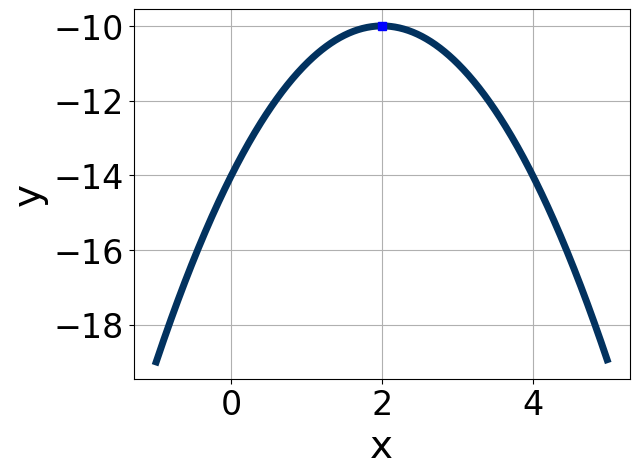
\includegraphics[width=0.5\textwidth]{../Figures/quadraticGraphToEquationB.png}
\end{center}
\begin{enumerate}[label=\Alph*.]
\item \( a \in [-1.2, -0.9], \hspace*{5mm} b \in [-9, -4], \text{ and } \hspace*{5mm} c \in [-8, -7] \)
\item \( a \in [-1.2, -0.9], \hspace*{5mm} b \in [-9, -4], \text{ and } \hspace*{5mm} c \in [-24, -20] \)
\item \( a \in [0.9, 1.2], \hspace*{5mm} b \in [-9, -4], \text{ and } \hspace*{5mm} c \in [7, 11] \)
\item \( a \in [0.9, 1.2], \hspace*{5mm} b \in [8, 11], \text{ and } \hspace*{5mm} c \in [7, 11] \)
\item \( a \in [-1.2, -0.9], \hspace*{5mm} b \in [8, 11], \text{ and } \hspace*{5mm} c \in [-24, -20] \)

\end{enumerate} }
\litem{
Solve the quadratic equation below. Then, choose the intervals that the solutions belong to, with $x_1 \leq x_2$ (if they exist).\[ 12x^{2} -11 x -8 = 0 \]\begin{enumerate}[label=\Alph*.]
\item \( x_1 \in [-1.7, -1.3] \text{ and } x_2 \in [-0.18, 0.87] \)
\item \( x_1 \in [-7, -2.9] \text{ and } x_2 \in [16.61, 16.75] \)
\item \( x_1 \in [-23.3, -21.5] \text{ and } x_2 \in [22.61, 23.39] \)
\item \( x_1 \in [-1.1, 0.8] \text{ and } x_2 \in [0.88, 2.02] \)
\item \( \text{There are no Real solutions.} \)

\end{enumerate} }
\litem{
Write the equation of the graph presented below in the form $f(x)=ax^2+bx+c$, assuming  $a=1$ or $a=-1$. Then, choose the intervals that $a, b,$ and $c$ belong to.
\begin{center}
    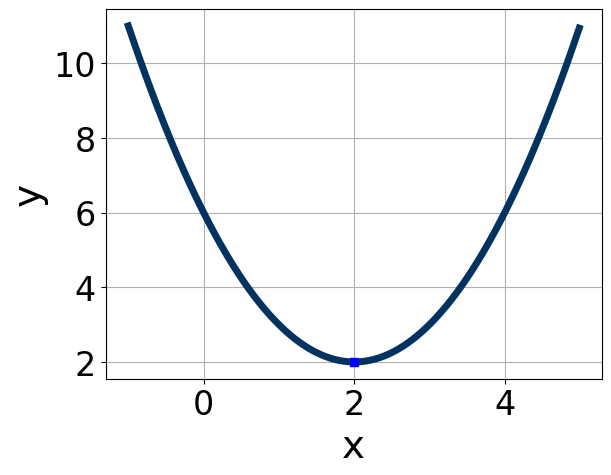
\includegraphics[width=0.5\textwidth]{../Figures/quadraticGraphToEquationCopyB.png}
\end{center}
\begin{enumerate}[label=\Alph*.]
\item \( a \in [1, 2], \hspace*{5mm} b \in [-10, -7], \text{ and } \hspace*{5mm} c \in [16, 21] \)
\item \( a \in [-4, 0], \hspace*{5mm} b \in [-10, -7], \text{ and } \hspace*{5mm} c \in [-14, -13] \)
\item \( a \in [-4, 0], \hspace*{5mm} b \in [-10, -7], \text{ and } \hspace*{5mm} c \in [-18, -15] \)
\item \( a \in [1, 2], \hspace*{5mm} b \in [7, 12], \text{ and } \hspace*{5mm} c \in [16, 21] \)
\item \( a \in [-4, 0], \hspace*{5mm} b \in [7, 12], \text{ and } \hspace*{5mm} c \in [-14, -13] \)

\end{enumerate} }
\litem{
Solve the quadratic equation below. Then, choose the intervals that the solutions belong to, with $x_1 \leq x_2$ (if they exist).\[ -12x^{2} +12 x + 3 = 0 \]\begin{enumerate}[label=\Alph*.]
\item \( x_1 \in [-0.38, -0.08] \text{ and } x_2 \in [1.04, 1.46] \)
\item \( x_1 \in [-14.52, -13.8] \text{ and } x_2 \in [1.84, 2.66] \)
\item \( x_1 \in [-16.73, -16.31] \text{ and } x_2 \in [17.1, 17.97] \)
\item \( x_1 \in [-1.88, -0.35] \text{ and } x_2 \in [-0.14, 0.68] \)
\item \( \text{There are no Real solutions.} \)

\end{enumerate} }
\litem{
Graph the equation below.\[ f(x) = -(x+4)^2 + 11 \]\begin{enumerate}[label=\Alph*.]
\begin{multicols}{2}\item 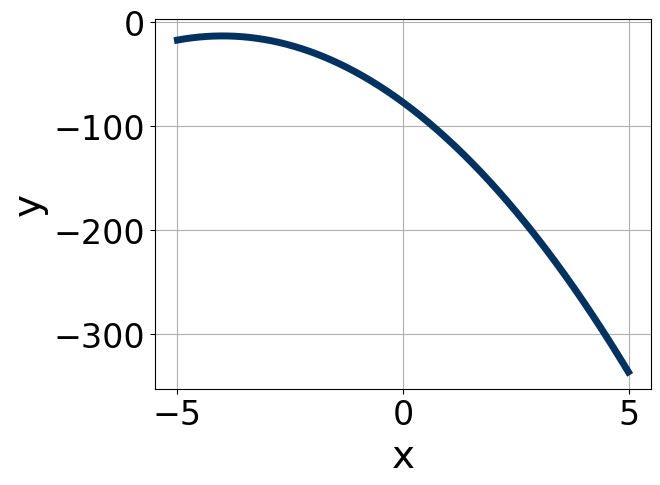
\includegraphics[width = 0.3\textwidth]{../Figures/quadraticEquationToGraphCopyAB.png}\item 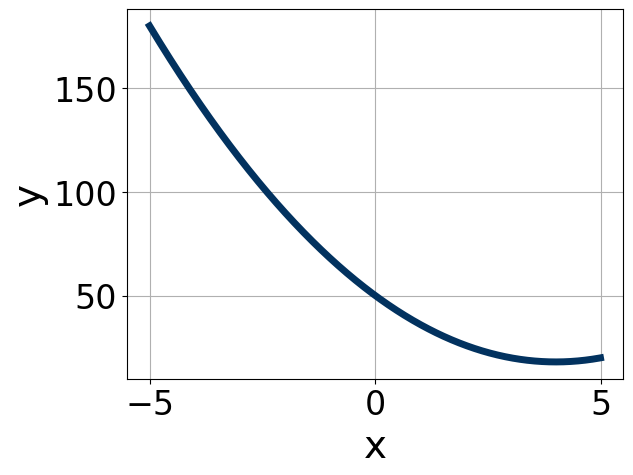
\includegraphics[width = 0.3\textwidth]{../Figures/quadraticEquationToGraphCopyBB.png}\item 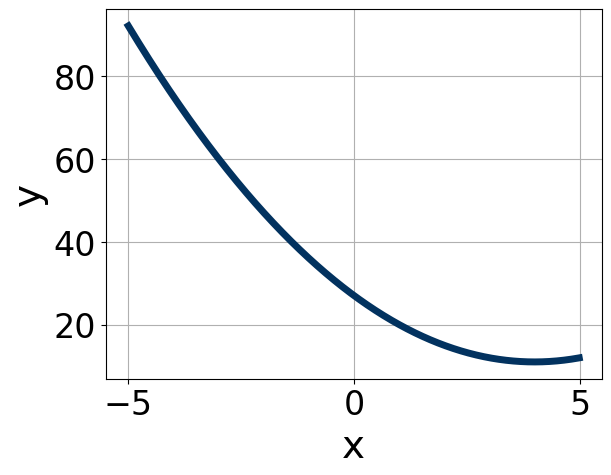
\includegraphics[width = 0.3\textwidth]{../Figures/quadraticEquationToGraphCopyCB.png}\item 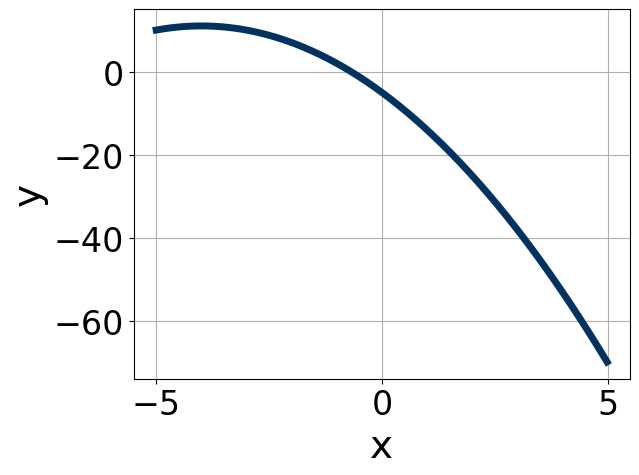
\includegraphics[width = 0.3\textwidth]{../Figures/quadraticEquationToGraphCopyDB.png}\end{multicols}\item None of the above.
\end{enumerate} }
\litem{
Solve the quadratic equation below. Then, choose the intervals that the solutions $x_1$ and $x_2$ belong to, with $x_1 \leq x_2$.\[ 25x^{2} +60 x + 36 = 0 \]\begin{enumerate}[label=\Alph*.]
\item \( x_1 \in [-3.11, -1.27] \text{ and } x_2 \in [-0.61, -0.55] \)
\item \( x_1 \in [-1.72, -0.17] \text{ and } x_2 \in [-1.38, -1.16] \)
\item \( x_1 \in [-30.83, -29] \text{ and } x_2 \in [-30.11, -29.9] \)
\item \( x_1 \in [-4.74, -3.44] \text{ and } x_2 \in [-0.41, -0.26] \)
\item \( x_1 \in [-6.13, -4.91] \text{ and } x_2 \in [-0.28, -0.16] \)

\end{enumerate} }
\litem{
Factor the quadratic below. Then, choose the intervals that contain the constants in the form $(ax+b)(cx+d); b \leq d.$\[ 24x^{2} -50 x + 25 \]\begin{enumerate}[label=\Alph*.]
\item \( a \in [0.04, 1.67], \hspace*{5mm} b \in [-30, -29], \hspace*{5mm} c \in [0.52, 1.5], \text{ and } \hspace*{5mm} d \in [-20, -17] \)
\item \( a \in [2.27, 5.23], \hspace*{5mm} b \in [-8, 0], \hspace*{5mm} c \in [5.62, 6.91], \text{ and } \hspace*{5mm} d \in [-6, -2] \)
\item \( a \in [11.09, 13], \hspace*{5mm} b \in [-8, 0], \hspace*{5mm} c \in [1.22, 2.97], \text{ and } \hspace*{5mm} d \in [-6, -2] \)
\item \( a \in [1.97, 3.06], \hspace*{5mm} b \in [-8, 0], \hspace*{5mm} c \in [11.99, 13.01], \text{ and } \hspace*{5mm} d \in [-6, -2] \)
\item \( \text{None of the above.} \)

\end{enumerate} }
\litem{
Factor the quadratic below. Then, choose the intervals that contain the constants in the form $(ax+b)(cx+d); b \leq d.$\[ 36x^{2} -65 x + 25 \]\begin{enumerate}[label=\Alph*.]
\item \( a \in [-0.36, 1.56], \hspace*{5mm} b \in [-47, -43], \hspace*{5mm} c \in [-2.5, 1.8], \text{ and } \hspace*{5mm} d \in [-20, -14] \)
\item \( a \in [3.97, 4.73], \hspace*{5mm} b \in [-5, -3], \hspace*{5mm} c \in [8.4, 10.1], \text{ and } \hspace*{5mm} d \in [-9, -2] \)
\item \( a \in [1.64, 2.78], \hspace*{5mm} b \in [-5, -3], \hspace*{5mm} c \in [16.7, 19.4], \text{ and } \hspace*{5mm} d \in [-9, -2] \)
\item \( a \in [11.45, 12.43], \hspace*{5mm} b \in [-5, -3], \hspace*{5mm} c \in [1.4, 5.9], \text{ and } \hspace*{5mm} d \in [-9, -2] \)
\item \( \text{None of the above.} \)

\end{enumerate} }
\litem{
Graph the equation below.\[ f(x) = (x-1)^2 - 10 \]\begin{enumerate}[label=\Alph*.]
\begin{multicols}{2}\item 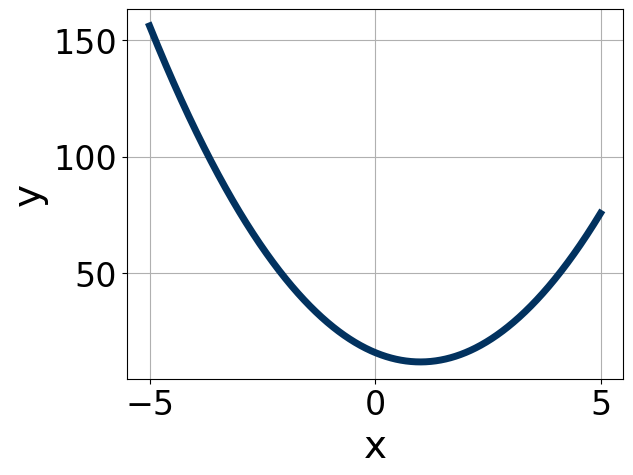
\includegraphics[width = 0.3\textwidth]{../Figures/quadraticEquationToGraphAB.png}\item 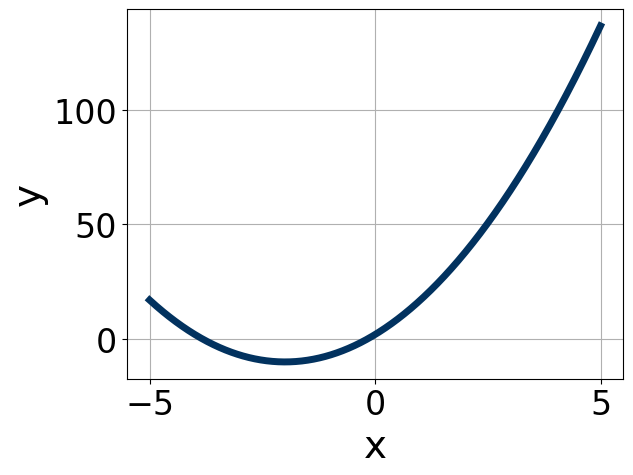
\includegraphics[width = 0.3\textwidth]{../Figures/quadraticEquationToGraphBB.png}\item 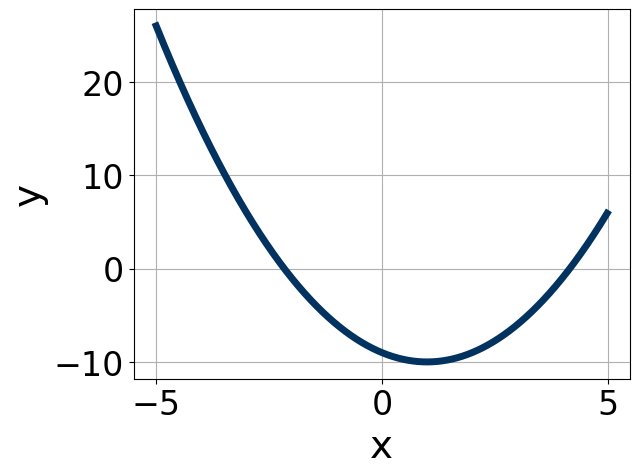
\includegraphics[width = 0.3\textwidth]{../Figures/quadraticEquationToGraphCB.png}\item 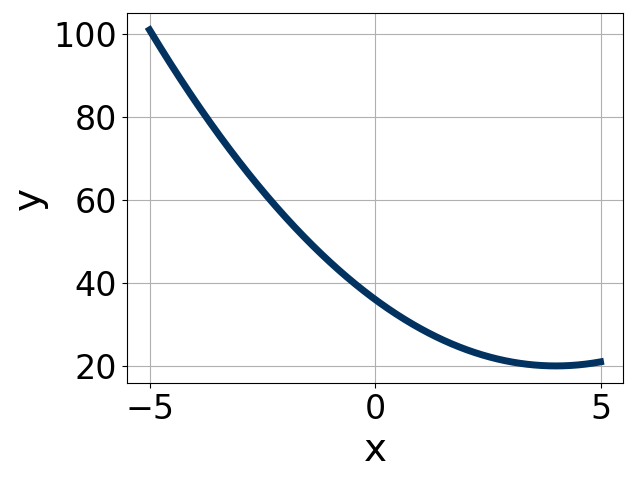
\includegraphics[width = 0.3\textwidth]{../Figures/quadraticEquationToGraphDB.png}\end{multicols}\item None of the above.
\end{enumerate} }
\end{enumerate}

\end{document}